\section{Lecture 1: January 14, 2025}

    \subsection{Introduction to Fine-Grained Complexity}
    
        We hope to precisely understand the complexity of several algorithmic problems beyond the coarse information given by standard complexity classes like \(\com{P}\) and \(\com{NP}\). A central theme is proving lower bounds for the complexity of algorithms; this is a difficult task in general. Here, reductions are an essential tool.
        \\
        \\
        The high-level idea behind fine-grained complexity is to explain hardness, or the lack of algorithmic progress, on fundamental computational problems by giving reductions from well-studied problems. Recall the \(\com{P}\) v. \(\com{NP}\) problem. Loosely, problems in \(\com{P}\) are ``easy,'' to solve, and problems in \(\com{NP}\) are ``easy'' to verify positive answers to. The hardest problems in \(\com{NP}\), the \(\com{NP}\)-complete problems, do not admit polynomial-time algorithms unless \(\com{P}=\com{NP}\). To show that a problem is \(\com{NP}\)-complete, we show that it is in \(\com{NP}\), and exhibit a polynomial-time reduction from a known \(\com{NP}\)-complete problem. We assume familiarity with the technical definitions and implications, and defer the reader to \cite{hopcroft2001introduction,sipser2012introduction} for details.
        \\
        \\
        The theory behind \(\com{NP}\)-completeness is robust and quite nice. But, we'd like finer results. Knowing whether a problem is in \(\com{P}\) or not doesn't really narrow down how efficiently we can solve it in practice. Even quadratic-time algorithms may be inefficient in production.
        \\
        \\
        These ideas motivate fine-grained complexity. Here, we start by taking a well-studied problem, say \(L_1\), and making a precise conjecture about the running time of optimal algorithms for \(L_1\). Then, we give an efficient reduction from \(L_1\) to a problem \(L_2\), for which we are showing hardness. We start by providing some hypotheses corresponding to certain problems, and later, we'll show fairly precise running time bounds for problems in \(\com{P}\).
        \begin{example}
            Under certain assumptions, there is no \(O(n^{2-\epsilon})\)-time algorithm for the \prob{Edit Distance} problem. This matches the \(O(n^2)\) dynamic programming algorithm.
        \end{example}
        \pagebreak
        \begin{compprob}[\(k\)-\textsc{SAT}] \label{prob:ksat}
            \vphantom
            \\
            \begin{itemize}
                \item Given a CNF formula \(\varphi\) with \(k\) literals in each clause,
                \item Decide: Does there exist a satisfying assignment?
            \end{itemize}
        \end{compprob}
        \begin{hypothesis}{\Stop\,\,\cite{impagliazzo2001ksatcomplexity} Exponential Time Hypothesis (ETH)}{ETH}
            The \(3\)-\prob{SAT} problem takes \(2^{\Omega(n)}\) time.
        \end{hypothesis}
        \begin{remark*}
            Note that \(\com{P}\neq\com{NP}\) asserts that \(3\)-\prob{SAT} has no polynomial-time algorithm, whereas ETH asserts that \(3\)-\prob{SAT} has no subexponential-time algorithm. Hence, ETH implies \(\com{P}\neq\com{NP}\).
        \end{remark*}
        \begin{hypothesis}{\Stop\,\,\cite{impagliazzo2001ksatcomplexity,impagliazzo2001stronglyexp} Strong Exponential Time Hypothesis (SETH)}{SETH}
            For every \(\epsilon>0\), there exists \(k\in\mathbb{Z}^+\) such that there is no \(O\left(2^{(1-\epsilon)n}\right)=O((2-\epsilon)^n)\)-time algorithm for \(k\)-\prob{SAT}.
        \end{hypothesis}
        \begin{remark*}
            SETH, at a high level, claims that \(2^n\)-time is essentially optimal for \(k\)-\prob{SAT} with large \(k\).
        \end{remark*}
        \begin{remark*}
            In \cite{impagliazzo2001ksatcomplexity,impagliazzo2001stronglyexp}, ETH and SETH are instead stated as follows. Let
            \begin{equation*}
            s_k=\inf\left\{\delta>0: \exists \text{ an algorithm to solve }k\textsc{-SAT}\text{ in }O^*\left(2^{\delta n}\right)\text{ time}\right\}.
            \end{equation*}
            ETH is the statement that for \(k\geq3\), \(s_k>0\). Assuming ETH, \(s_k\) is increasing infinitely often, \cite{impagliazzo2001stronglyexp}. Let \(s_\infty=\lim_{k\to\infty} s_k\). Then, SETH is the statement that \(s_\infty=1\).
        \end{remark*}
        \begin{compprob}[\(k\)-\textsc{Sum}] \label{prob:ksum}
            \vphantom
            \\
            \begin{itemize}
                \item Given arrays \(A_1,\ldots,A_k\) each with \(n\) integers in \([-n^c,n^c]\),
                \item Decide: Does there exist \(a_1\in A_1,\ldots, a_k\in A_k\) such that \(a_1+\cdots+a_k=0\)?
            \end{itemize}
            Some variants include assuming that \(A_1=\cdots=A_k\), or wanting to find \(a_1\in A_1,\ldots, a_k\in A_k\) where \(a_1+\cdots+a_{k-1}=a_k\).
        \end{compprob}
        \vphantom
        \\
        \\
        A naive algorithm for \(k\textsc{-Sum}\) is to try all possible choices \(a_i\) and verify the sum. This gives rise to an \(O(n^k)\)-time algorithm.
        \begin{question*}
            Can we do better?
        \end{question*}
        \begin{answer*}
            Yes, we can!
        \end{answer*} 
        \vphantom
        \\
        \\
        For now, let \(k=3\). Consider the following, slightly better, algorithm.
        \begin{algorithm}[H] 
            \begin{algorithmic}[1]
                \Procedure{3-Sum-Better}{$A_1,A_2,A_3$} 
                    \State \(S\gets \{a_1+a_2:a_1\in A,a_2\in A_2\}\) \Comment{\(O(n^2)\)}
                    \State Sort \(A_3\). \Comment{\(O(n\log n)\)}
                    \For{\(s\in S\)} \Comment{\(O(n^2\log n)\)}
                        \If{\(-s\in A_3\)} \Return \(\var{true}\) 
                        \EndIf
                    \EndFor
                    \State \Return \(\var{false}\)
                \EndProcedure 
            \end{algorithmic}
            \caption{Better \(3\textsc{-Sum}\)}
            \label{alg:better-3-sum}
        \end{algorithm}
        \vphantom
        \\
        \\
        Algorithm~\ref{alg:better-3-sum} takes \(O(n^2\log n)\) time, using binary search on the sorted array \(A_3\).
        \pagebreak
        \begin{question*}
            Can we do better?
        \end{question*}
        \begin{answer*}
            Yes, we can!
        \end{answer*} 
        \vphantom
        \\
        \\
        Our first example of a helpful reduction is as follows. Given a \(3\textsc{-Sum}\) instance with arrays of length \(n\), we can construct \(n\) \(2\textsc{-Sum}\) instances. This procedure gives us an \(O(n^2)\) algorithm for \(3\textsc{-Sum}\), which we describe in Algorithm~\ref{alg:best-3-sum}.
        \begin{algorithm}[H] 
            \begin{algorithmic}[1]
                \Procedure{3-Sum-Better}{$A_1,A_2,A_3$} 
                    \State Sort \(A_1\) and \(A_2\).
                    \For{\(a_3\in A_3\)}
                        \State \(A_2+a_3\gets [a_{2,1}+a_3,\ldots,a_{2,n}+a_3]\) 
                        \If{\Call{2-Sum}{$A_1,A_2+a_3$}} \Return \(\var{true}\)
                        \EndIf
                    \EndFor
                    \State \Return \(\var{false}\)
                \EndProcedure 
            \end{algorithmic}
            \caption{Best \(3\textsc{-Sum}\)}
            \label{alg:best-3-sum}
        \end{algorithm}
        \vphantom
        \\
        \\
        Sorting takes \(O(n\log n)\) time. Then, we can \(n\) calls of \(2\textsc{-Sum}\) that each take \(O(n)\) time since the arrays are sorted. Therefore, Algorithm~\ref{alg:best-3-sum} runs in \(O(n^2)\) time. We have the following hypothesis.
        \begin{hypothesis}{\Stop\,\,No \(O(n^{2-\epsilon})\)-Time Algorithm for \(3\)-\textsc{Sum}}{nobetterthanquadratictime3sum}
            For every \(\epsilon>0\), there is no \(O\left(n^{2-\epsilon}\right)\)-time algorithm for \(3\)-\textsc{Sum}.
        \end{hypothesis}
        

\pagebreak

\section{Lecture 2: January 16, 2025}

    \subsection{Fine-Grained Complexity II}

        Now, we introduce a new problem. 
        \begin{compprob}[\textsc{All Pairs Shortest Path (APSP)}] \label{prob:apsp}
            \vphantom
            \\
            \begin{itemize}
                \item Given a weighted graph \(G=(V,E,w)\) on \(n\) vertices,
                \item Find: The lengths of the shortest paths \(d(v_i,v_j)\) between every \(v_i,v_j\in V\).
            \end{itemize}
        \end{compprob}
        \vphantom
        \\
        \\
        One way to solve \textsc{APSP} is to run Dijkstra's algorithm on each vertex. Recall that Dijkstra's algorithm finds a single-source shortest path tree. We could also similarly use the Floyd-Warshall dynamic programming algorithm which we introduce below. 
        \\
        \\
        Let \(D_k[i,j]\) store the length of the shortest path from \(v_i\) to \(v_j\), with the restriction that the path only passes through \(v_1,\ldots,v_k\).
        \begin{example}
            To illustrate this notion, consider the below graph.
            \begin{figure}[H]
                \begin{center}
                    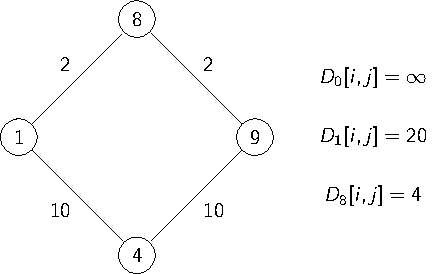
\includegraphics{Graphics/Figures/floyd_warshall/table_example.pdf}
                \end{center}
                \caption{Example of \(D_k[i,j\)]}
                \label{fig:example-floyd-warshall-table}
            \end{figure}
        \end{example}
        \pagebreak
        \vphantom
        \\
        \\
        Illustrated in Figure~\ref{fig:floyd-warshall-table-update}, the idea behind Floyd-Warshall is to build \(D_k\) from \(D_{k-1}\), noting that either
        \begin{enumerate}
            \item the shortest path from \(v_i\) to \(v_j\) only using \(v_1,\ldots,v_k\) uses \(v_k\), or 
            \item it does not.
        \end{enumerate}
        \begin{figure}[H]
            \begin{center}
                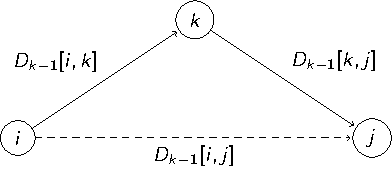
\includegraphics{Graphics/Figures/floyd_warshall/table_update.pdf}
            \end{center}
            \caption{Update of \(D_k[i,j\)]}
            \label{fig:floyd-warshall-table-update}
        \end{figure}
        \vphantom
        \\
        \\
        From this basic idea, we get a simple algorithm.
        \begin{algorithm}[H] 
            \begin{algorithmic}[1]
                \Require \(G=(V,E,w)\).
                \Procedure{Floyd\_Warshall}{$E$} 
                    \State \(D_0\gets\begin{cases}
                        0 & i=j \\
                        w_{i,j} & i\neq j, (v_i,v_j)\in E \\
                        \infty & (v_i,v_j)\nin E
                    \end{cases}\)
                    \For{\(k\in\{1,\ldots,n\}\)}
                        \For{\(i\in\{1,\ldots,n\}\)}
                            \For{\(j\in\{1,\ldots,n\}\)}
                                \State \(D_{k}[i,j]=\min\{D_{k-1}[i,k]+D_{k-1}[k,j], D_{k-1}[i,j]\}\)
                            \EndFor
                        \EndFor
                    \EndFor
                    \State \Return \(D_n\)\Comment{\(D_n[i,j]=d(v_i,v_j)\)}
                \EndProcedure 
            \end{algorithmic}
            \caption{Floyd-Warshall}
            \label{alg:floydwarshall}
        \end{algorithm}
        \vphantom
        \\
        \\
        It turns out that as far as we know, Algorithm~\ref{alg:floydwarshall} with complexity \(O(n^3)\) is the best we can do.
        \begin{hypothesis}{\Stop\,\,No \(O(n^{3-\epsilon})\)-Time Algorithm for \textsc{APSP}}{nobetterthancubictimeapsp}
            For every \(\epsilon>0\), there exists no \(O(n^{3-\epsilon})\)-time algorithm for \textsc{APSP}.
        \end{hypothesis}
        \pagebreak
        \vphantom
        \\
        \\
        We now turn to a new problem.
        \begin{compprob}[\textsc{Orthogonal Vectors (OV)}] \label{prob:ov}
            \vphantom
            \\
            \begin{itemize}
                \item Given two sets \(V=\{v_1,\ldots,v_n\}\subseteq\{0,1\}^d\) and \(W=\{w_1,\ldots,w_n\}\subseteq\{0,1\}^d\),
                \item Decide: Does there exist \(v_i\in W\) and \(w_j\in W\) such that \(\iprod{v_i}{w_j}=\sum_{k=1}^d v_i[k]w_j[k]=0\)?
            \end{itemize}
        \end{compprob}
        \vphantom
        \\
        \\
        The naive algorithm is to compare every pair, compute the inner products, and compare to \(0\). We have \(n^2\) inner products to compute, and each takes \(d\) time, so the naive algorithm takes \(O(dn^2)\) time. Think of \(d=\log^k(n)\) for some \(k\). In this case, \(O(dn^2)=O(n^2\log^k(n))=\tilde{O}(n^2)\).
        \begin{hypothesis}{\Stop\,\,No \(O(n^{2-\epsilon})\)-Time Algorithm for \textsc{OV}}{nobetterthanquadratictimeov}
            For every \(\epsilon>0\), there exists no \(O(n^{2-\epsilon})\)-time algorithm for \textsc{OV} with \(d=\polylog(n)\).
        \end{hypothesis}
        \vphantom
        \\
        \\
        So far, we have \(5\) hypotheses; what are the relations herein? We'll attack this question after a brief interlude on reductions.
        \\
        \\
        We write \(L_1\leq L_2\) if problem \(L_1\) reduces to problem \(L_2\); that is, \(L_1\) is no harder than \(L_2\); and if \(L_1\) is hard, then \(L_2\) is hard. Equivalently, if \(L_2\) is easy, then \(L_1\) is easy. Consider the following definition, making precise the notion of a ``fine-grained reduction.''
        \begin{definition}{\Stop\,\,\cite{williams2019finegrained} Fine-Grained Reductions}{finegrainedreductions}
            Suppose \(L_1\) and \(L_2\) are computational problems. Let \(\ell_1=\ell_1(n)\) and \(\ell_2=\ell_2(n)\) be associated conjectured optimal runtime bounds. Then, \(L_1\) \((\ell_1,\ell_2)\)-reduces to \(L_2\) if for every \(\epsilon>0\), there exists \(\delta>0\) and an algorithm \(R\) for \(L_1\) running in time \(O(\ell_1(n)^{1-\delta})\) and making \(q\) calls to an oracle for \(L_2\) on inputs of size \(n_1,\ldots,n_q\) where
            \begin{equation*}
                \sum_{i=1}^q \ell_2(n_i)^{1-\epsilon}\leq O(\ell_1(n)^{1-\delta}).
            \end{equation*}
            We write \(L_1\leq_{\ell_1,\ell_2} L_2\). If both \(L_1\leq_{\ell_1,\ell_2} L_2\) and \(L_2\leq_{\ell_1,\ell_2} L_1\), we say \(L_1=_{\ell_1,\ell_2}L_2\).
        \end{definition}
        \pagebreak
        \begin{theorem}{\Stop\,\,\cite{williams2005twoconstraintsat} SETH \(\implies\) OV}{sethimpliesov}
            Hypothesis~\ref{hyp:SETH} implies Hypothesis~\ref{hyp:nobetterthanquadratictimeov}.
            \begin{proof}
                Using Definition~\ref{def:finegrainedreductions}, we can restate this theorem as follows: for every \(k\in\mathbb{Z}^+\), \(k\)-\textsc{SAT} \((2^n,n^2)\)-reduces to \textsc{OV} with \(d=\polylog(n)\). We exhibit such a reduction, which will be of exponential-time.
                \\
                \\
                Let \(\varphi(x_1,\ldots,x_n)=\bigwedge_{j=1}^m C_j\) be our \(k\)-\textsc{SAT} instance, with each \(C_j\) a \(k\)-clause. Partition \(X=\{x_i\}_{i=1}^n\) into \(X_1=\{x_1,\ldots,x_{\frac{n}{2}}\}\) and \(X_2=\{x_{\frac{n}{2}+1},\ldots,x_n\}\). Consider the \(N=2^\frac{n}{2}\) assignments to each of \(X_1\) and \(X_2\) independently. Then, let \(V_1,V_2\subseteq\{0,1\}^m\). For an assignment \(a_1\) to literals in \(X_1\), \(v_{a_1}\in V_1\) is defined by
                \begin{equation*}
                    v_{a_1}[j]=\begin{cases}
                    0 & a_1\text{ satisfies }C_j \\
                    1 & \text{otherwise}
                    \end{cases}.
                \end{equation*}
                Define \(v_{a_2}\in V_2\) similarly corresponding to \(a_2\) with literals in \(X_2\). We claim that \(\iprod{v_{a_i}}{v_{a_2}}=0\) if and only if \([a_1,a_2]\) is a satisfying assignment. Note that \(m=O(n^k)=O((2\log_2N)^k)=O(\log^kN)\), where \(N=2^\frac{n}{2}\). A \(O\left(N^{2-\epsilon}\right)\)-time algorithm for \textsc{OV} would then imply an \(O\left(N^{2-\epsilon}\right)=O\left(\left(2^\frac{n}{2}\right)^{2-\epsilon}\right)=O\left(2^{\left(1-\frac{\epsilon}{2}\right)n}\right)\)-time algorithm for \(k\)-\textsc{SAT}. 
            \end{proof}
        \end{theorem}
        \begin{example}
            To illustrate the reduction in the proof of Theorem~\ref{thm:sethimpliesov}, consider \(k\textsc{-SAT}\) with \(n=6\), \(m=3\), and \(k=3\) and formula
            \begin{equation*}
                \varphi(x_1,\ldots,x_6)=(x_1\vee\neg x_2\vee x_6)\wedge(x_2\vee x_3\vee x_4)\wedge (\neg x_4\vee \neg x_3\vee x_6).
            \end{equation*}
            For \(a_1=[0,1,0]\), we have \(v_{a_1}=[1,0,0]\in V_1\) and for \(a_2=[0,1,1]\), we have \(v_{a_2}=[0,1,0]\in V_2\). Indeed \(\varphi(a_1,a_2)=1\) and \(\iprod{v_{a_1}}{v_{a_2}}=0\).
        \end{example}

\pagebreak
    
\section{Lecture 3: January 21, 2025}

    \subsection{Graph Diameter}

        Consider the following problem.
        \begin{compprob}[Graph Diameter] \label{prob:graphdiam}
            \vphantom
            \\
            \begin{itemize}
                \item Given a graph \(G=(V,E,w)\), 
                \item Find: \(\max_{u,v\in V}d(u,v)\) where \(d(u,v)\) is the shortest path distance between \(u,v\in V\).
            \end{itemize}
            
        \end{compprob}
        \vphantom
        \\
        \\
        An easy algorithm is to run Floyd-Warshall and output the largest distance found. This takes \(O(n^3)\) time.
        \begin{theorem}{\Stop\,\,\cite{roditty2013fast} \textsc{OV} Reduction to \textsc{GraphDiameter}}{ovtographdiam}
            The \textsc{OV} problem \((n^2,n^2)\)-reduces to \textsc{GraphDiameter} on undirected, unweighted graphs with \(O(n)\) vertices and \(\tilde{O}(n)\) edges.
            \begin{proof}
                Let \(V=[v_1',\ldots,v_n']\subseteq\{0,1\}^d\) and \(W=[w_1',\ldots,w_n']\subseteq\{0,1\}^d\)
            \end{proof}
        \end{theorem}
        \begin{remark*}
            Theorem~\ref{thm:ovtographdiam} immediately shows that assuming Hypothesis~\ref{hyp:nobetterthanquadratictimeov} or SETH, there exists no \(O\left(n^{2-\epsilon}\right)\)-time algorithm to \(\left(\frac{3}{2}-\delta\right)\)-approximate \textsc{GraphDiameter} for all \(\epsilon,\delta>0\).
        \end{remark*}
        \adit{Finish this! I was very tired during lecture...}



\pagebreak

\section{Lecture 4: January 23, 2025}

    \subsection{Smarter \(k\)-SAT, Part I}

        [Monien-Speckenmeyer, 1985]

        We've shown a \(O(1.913^n)\) algorithm for \(3\)-SAT. Can we do better? Yes, we can! Consider a clause \(C=x_1\vee x_2\vee x_2\). Note that
        \begin{equation*}
            C=x_1\vee x_2\vee x_2\iff x_1\vee(\neg x_1\wedge x_2)\vee(\neg x_1\wedge \neg x_2\wedge x_3).
        \end{equation*}
        We can think of the above formula as either setting the truth of one, two, or three literals. This gives rise to a modification of the previous recursive algorithm, making \(3\) recursive calls. This gives us the recurrence \(T(n)=T(n-1)+T(n-2)+T(n-3)+\poly(n)=O^*(\alpha^n)\) where \(\alpha\) is the unique real root to \(\alpha^n-\alpha^{n-1}-\alpha^{n-2}-\alpha^{n-3}=0\), or equivalently, \(\alpha^3-\alpha^2-\alpha-1\). Here, \(\alpha\leq 1.84\). So, \(T(n)=(1.84^n)\).
        \\
        \\
        We now show how to reduce \(k\)-\textsc{SAT} to \(k-1\)-\textsc{SAT} where \(k\geq4\). Take the \(k\)-\textsc{SAT} formula
        \begin{equation*}
            \varphi=\bigwedge_{j=1}^m C_j.
        \end{equation*}
        We will map each clause \(C_j\) in \(\varphi\) to the conjunction of a \(k-1\)-clause, and a \(3\)-clause. We'll introduce a new variable \(y\) each time. Say
        \begin{equation*}
            C_j=(x_1^j,\ldots,x_k^j)\mapsto (x_1^j,\ldots,x_{k-2}^j\vee y)\wedge (\neg y\vee x_{k-1}^j\vee x_k^j).
        \end{equation*}
        Now, we consider local search algorithms for \(3\)-\textsc{SAT} [Spielman's Notes, \cite{schoning1999probabilisticksat}]. Here, we harness the power of randomness.
        \begin{algorithm}[H] 
            \begin{algorithmic}[1]
                \Procedure{Sch\"oning\_SAT\_Framework}{$\varphi,\beta_n$} 
                    \State Guess a uniformly random assignment to \(\vec{a}\in\{0,1\}^n\) to \(\varphi\).
                    \For{\(j\in\{1,\ldots,\beta_n\}\)}
                        \If{\(\varphi\) is satisfied by \(\vec{a}\)}
                            \State \Return \(\vec{a}\)
                        \Else
                            \State Choose an unsatisfied clause \(C\) in \(\varphi\), and choose a variable \(x_i\) in \(C\) uniformly at random.
                            \State Flip the assignment \(a_i\) to \(x_i\) in \(\vec{a}\).
                        \EndIf
                    \EndFor
                    \State \Return \(\vec{a}\)
                \EndProcedure 
            \end{algorithmic}
            \caption{Sch\"oning SAT}
            \label{alg:schoningsat}
        \end{algorithm}
        \begin{example}
            Say \(C=(x_1,x_2,x_3)\) with \(a_1=0\), \(a_2=0\), and \(a_3=0\). Since \(C\) is unsatisfied, we can flip one of the literals uniformly at random to satisfy \(C\).
        \end{example}
        \vphantom
        \\
        \\
        Importantly, how do we choose \(\beta_n\)? Suppose that the initial assignment \(\vec{a}\) agrees with the satisfying assignment \(\vec{a}^*\) on a ``decent'' fraction of coordinates with ``decent'' probability. The steps in the loop can be thought of as doing a random walk on \(\{0,1\}^n\). At each step, \(\vec{a}\) gets closer to \(\vec{a}^*\) with probability at least \(\frac{1}{3}\) since at least one variable in each unsatisfied clause differs between \(\vec{a}\) and \(\vec{a}^*\). 
        \\
        \\
        For ``Easy''-Sch\"oning, take \(\beta_n=n\). Say \(u\) is the number of coordinates in which \(\vec{a}\) and \(\vec{a}^*\) disagree. Then,
        \begin{align*}
            \Pr[\text{success}]&\geq \sum_{i=0}^n \Pr[u=i]\Pr[\text{first }i\text{ choices match}] \\
            &=\sum_{i=0}^n \frac{1}{2^n}\binom{n}{i}\Pr[\text{first }i\text{ choices match}] \\
            &\geq\frac{1}{2^n}\sum_{i=0}^n\binom{n}{i}\frac{1}{3^i} \\
            &=\frac{1}{2^n}\left(1+\frac{1}{3}\right)^n \\
            &=\left(\frac{2}{3}\right)^n.
        \end{align*}
        Intuitively, we sample a random assignment \(\vec{a}\) which disagrees in \(i\) coordinates from \(\vec{a}^*\). We want to keep flipping assigments so that \(\vec{a}=\vec{a}^*\). The algorithm succeeds with probability at least \(\left(\frac{2}{3}\right)^n\). So, we can repeat Algorithm~\ref{alg:schoningsat} roughly \(\left(\frac{3}{2}\right)^n\) with \(\beta=n\) times to find a solution with high probability.
        \adit{FINISH THIS! (and undertsnad this fully!)}
        \\
        \\
        We now present another result: the sparsification lemma. Morally, we can reduce solving a \(k\)-\textsc{SAT} instance with \(n\) variables to solving several \(k\)-\textsc{SAT} instances each with \(n\) variables \(O(n)\) clauses. Informally, ``every \(k\)-\textsc{SAT} formula has \(O(n)\) clauses.''
        \begin{theorem}{\Stop\,\,The Sparsification Lemma}{sparsificationlemma}
            Let \(\epsilon>0\) and \(k\geq3\). Then, there is a \(2^{\epsilon n}\poly(n)\)-time algorithm that takes a \(k\)-\textsc{SAT} formula \(\varphi\) on \(n\) variables as input and produces \(2^{\epsilon n}\) \(k\)-\textsc{SAT} formulas \(\varphi_1,\ldots,\varphi_{2^{\epsilon n}}\), each of which has \(n\) variables and \(n\left(\frac{k}{\epsilon}\right)^{O(k)}=O(n)\) clauses. Furthermore, \(\varphi\) is satisfiable if and only if \(\bigvee_i \varphi_i\) is satisfied.
        \end{theorem}
        \vphantom
        \\
        \\
        With the help of Theorem~\ref{thm:sparsificationlemma}, we can show that the ``strong'' exponential time hypothesis indeed implies the exponential time hypothesis.
        \adit{TODO! HW.}
        % We called Hypothesis~\ref{hyp:SETH} the ``strong'' exponential time hypothesis. But, does Hypothesis~\ref{hyp:SETH} imply Hypothesis~\ref{hyp:ETH}, the exponential time hypothesis?

\pagebreak

\section{Lecture 5: January 28, 2025}

    \subsection{Smarter \(k\)-SAT, Part II}

        Now, what if we apply the framework behind Algorithm~\ref{alg:schoningsat} with \(\beta_n=3n\)? Let's analyze the probability that 
        \begin{enumerate}
            \item the initial assignment \(\vec{a}\) disagrees with \(\vec{a}^*\) on exactly \(i\) coordinates, and
            \item the first \(3i\) steps of the walk include at least \(2i\) ``good'' choices.
        \end{enumerate}
        For (1), the analysis is very similar to ``Easy''-Sch\"oning. First, recall that for \(i\geq 2\),
        \begin{equation*}
            \binom{3i}{i}\geq \frac{1}{\sqrt{5i}}\frac{3^{3i}}{2^{2i}}
        \end{equation*}
        by Stirling's approximation. Then,
        \begin{align*}
            \Pr[\text{at least }2i\text{ of the first }3i\text{ choices are good}]&\geq\binom{3i}{i}\left(\frac{1}{3}\right)^{2i}\left(\frac{2}{3}\right)^i \\
            &\geq \frac{1}{\sqrt{3i}}\frac{3^{3i}}{2^{2i}}  \left(\frac{1}{3}\right)^{2i}\left(\frac{2}{3}\right)^i
        \end{align*}
        Then,
        \begin{align*}
            \Pr[\text{success}]&\geq \sum_{i=0}^n\Pr[u=i]\Pr[\text{at least }2i\text{ of the first }3i\text{ choices are good}] \\
            &\geq \frac{1}{2^n}\sum_{i=0}^n \binom{n}{i}\binom{3i}{i}  \left(\frac{1}{3}\right)^{2i}\left(\frac{2}{3}\right)^i \\
            &\geq \frac{1}{2^n}\sum_{i=0}^n \binom{n}{i}\frac{1}{\sqrt{3i}}\frac{3^{3i}}{2^{2i}}  \left(\frac{1}{3}\right)^{2i}\left(\frac{2}{3}\right)^i \\
            &\geq \frac{1}{2^n\sqrt{5n}}\sum_{i=0}^n\binom{n}{i}\frac{1}{\sqrt{3i}}\frac{3^{3i}}{2^{2i}}  \left(\frac{1}{3}\right)^{2i}\left(\frac{2}{3}\right)^i \\
            &=\frac{1}{2^n\sqrt{5n}}\sum_{i=0}^n\binom{n}{i}\frac{1}{2^i} \\
            &=\frac{1}{2^n\sqrt{5n}}\left(1+\frac{1}{2}\right)^n \\
            &=\frac{1}{\sqrt{5n}}\left(\frac{3}{4}\right)^n.
        \end{align*}
        Proceeding similarly, we can run Algorithm~\ref{alg:schoningsat} roughly \(O^*\left(\frac{4}{3}\right)^n\) times with \(\beta=3n\) times to find a solution with high probability.
        \begin{question*}
            Is this optimal?
        \end{question*}
        \begin{answer*}
            No! But, we'll end here.
        \end{answer*}

        
\section{Lecture 6: January 30, 2025}

    \subsection{Nontrivial Nondeterministic Algorithms: SETH and Other Assumptions}

        Consider the following definition.
        \begin{definition}{\Stop\,\,NTIME}{ntime}
            A language \(L\subseteq\{0,1\}^n\) is in \(\NTIME(f_n)\) if there exists an algorithm \(M\) such that for \(x\in\{0,1\}^*\) with \(|x|=n\), \(M\) runs in time \(f(n)\) and
            \begin{enumerate}
                \item if \(x\in L\), then there exists \(w\in\{0,1\}^*\) with \(M(x,w)\) accepting, and
                \item if \(x\nin L\), for all \(w\in\{0,1\}^*\), \(M(x,w)\) is rejecting.
            \end{enumerate}
        \end{definition}
        \begin{remark*}
            The familiar complexity class \(\com{NP}\) is given by
            \begin{equation*}
                \com{NP}=\bigcup_{k\in\mathbb{N}}\NTIME(n^k).
            \end{equation*}
        \end{remark*}
        \vphantom
        \\
        \\
        Herein, we reference \cite{carmosino2016nseth}. Recall that \(k\textsc{-SAT}\in\com{NP}\).
        \begin{question*}
            Can we say anything about verifying that a \(k\)\textsc{-SAT} formula is unsatisfiable?
        \end{question*}
        \begin{hypothesis}{\Stop\,\,NSETH}{nseth}
            For every \(\epsilon>0\), there exists \(k\) with \(\bar{k\textsc{-SAT}}\nin\NTIME\left(2^{(1-\epsilon)n}\right)\).
        \end{hypothesis}
        \begin{remark*}
            NSETH essentially hypothesizes that \(k\textsc{-SAT}\) has no nontrivial verification algorithm.
        \end{remark*} 
        \vphantom
        \\
        \\
        The key takeways of \cite{carmosino2016nseth} are that
        \begin{enumerate}
            \item assuming NSETH, \(\bar{k\textsc{-SAT}}\) does not have nontrivial nondeterministic algorithms,
            \item \(\bar{3\textsc{-Sum}}\) and \(\bar{\textsc{APSP}}\) do have nontrivial nondeterministic algorithms, and
            \item assuming (1), (2) and NSETH, there is no fine-grained reduction from \(k\textsc{-SAT}\) to \(3\textsc{-Sum}\) or \(\textsc{APSP}\), as opposed to the \(k\textsc{-SAT}\) to \(\textsc{OV}\) reduction.
        \end{enumerate}
        
        \pagebreak

        Consider the following theorem.
        \begin{theorem}{\Stop\,\,\cite{carmosino2016nseth} Nondeterministically Solving \(\bar{3\textsc{-Sum}}\) in \(\tilde{O}(n^{\frac{3}{2}})\) Time}{n1.5nondetalgforbar3sum}
            There is a \(\tilde{O}\left(n^{\frac{3}{2}}\right)\)-time nondeterministic algorithm for \(\bar{3\textsc{-Sum}}\).
            \begin{proof}
                Take the variant of \(3\textsc{-Sum}\) where we are given a single list \(A=[a_1,\ldots,a_n]\) where \(a_i\in[-n^c,n^c]\), and we are to decide if there exist \(a_i,a_j,a_k\in A\) with \(a_i+a_j+a_k=0\). So, for \(\bar{3\textsc{-Sum}}\), we must verify that for all \(i,j,k\in\{1,\ldots,n\}\), \(a_i+a_j+a_k\neq0\). The witness is a triple \((p,t,S)\) where 
                \begin{enumerate}
                    \item \(p\) is a prime which is at most the \(n^{1.5\textsc{th}}\) prime number,
                    \item \(S=\{(i,j,k):a_i+a_j+a_j\equiv0\pmod{p}\}\), and
                    \item \(t\in\mathbb{Z}\cap[0,3cn^{1.5}\log n]\) such that \(t=|S|\).
                \end{enumerate}
                We wish to show that such a witness exists. Let \(R\) be the set of all pairs \(((i,j,k),p)\) where \(p\) is a prime which is at most the \(n^{1.5\textsc{th}}\) prime number and \(a_i+a_j+a_k\equiv0\pmod{p}\). Then, \(|R|\leq n^3\log(3n^c)\leq 3cn^3\log n\). There are \(n^3\) triples \((i,j,k)\), and \(3n^c\) gives an upper bound on the magnitude of \(a_i+a_j+a_k\), and the logarithm is an upper bound on the number of prime factors of this quantity. Now, by an averaging argument, there must exist \(p_0\) which is at most the \(n^{1.5\textsc{th}}\) prime number such that the number of pairs \(((i,j,k),p_0)\) is at most \(\frac{|R|}{n^{1.5}}\leq 3cn^{1.5}\log n\). We now show verification given input \(A\). First, check that for all \(r\in\{1,\ldots,t\}\),
                \begin{equation*}
                    a_{ir}+a_{jr}+a_{kr}\equiv0\pmod{p},\quad a_{ir}+a_{jr}+a_{kr}\neq0.
                \end{equation*}
                Then compute the number of triples summing to \(0\) modulo \(p\) compare this with \(t\). To compute all triple sums, map
                \begin{equation*}
                    A=[a_1,\ldots,a_n]\mapsto q_A(x)=\sum_{i}x^{a_i\bmod p}
                \end{equation*}
                and use the fast Fourier transform to compute \((q_A(x))^3\). If \(b_j\) is the coefficient of \(x^j\) in \((q_A(x))^3\), \(b_3\) is the number of triples in \(\{a_1\bmod p,\ldots,a_n\bmod p\}\) summing to \(j\). Now, since \(\deg (q_A(x))^3\leq 3(p-1)<3p\), we can just check
                \begin{equation*}
                    b_0+b_{p}+b_{2p}=t,
                \end{equation*}
                and accept if we have equality, and reject otherwise.
                \\
                \\
                For complexity, the first check for \(r\in\{1,\ldots,t\}\) takes time \(O(t)=O\left(n^{\frac{3}{2}}\log n\right)\). The fast Fourier transform computation takes time \(O(p\log p)=\tilde{O}\left(n^\frac{3}{2}\right)\) where \(p=O\left(n^{\frac{3}{2}}\log n\right)\). In short, our procedure takes \(O\left(n^{\frac{3}{2}}\log n\right)\), as desired.
            \end{proof}
        \end{theorem}